\documentclass[tikz]{standalone}
\usepackage{amsmath,amssymb}

\newcommand{\twovec}[2]{\ensuremath{\begin{pmatrix}{#1}\\{#2}\end{pmatrix}}}
\newcommand{\V}[1]{\vec{\mathbf{#1}}}
\usetikzlibrary{calc,patterns}
\tikzset{mydraw/.style={black,->}}
\tikzset{mynode/.style={scale=0.7}}

\begin{document}
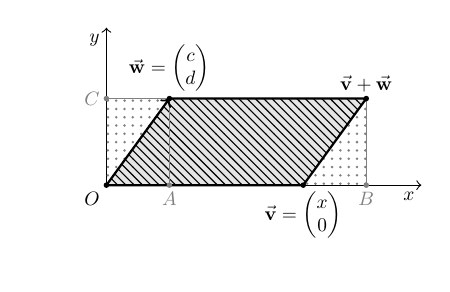
\begin{tikzpicture}
	\clip (-1,-1) rectangle (4,2);

	\coordinate (v) at (2.5, 0);
	\coordinate (wx) at (0.8, 0);
	\coordinate (wy) at (0, 1.1);
	\coordinate (w) at ($(wx) + (wy)$);
	\coordinate (vw) at ($(v) + (w)$);
	\coordinate (vwx) at ($(v) + (wx)$);

	\draw[mydraw] (0,0) -- (4,0) node[mynode,below left] {\(x\)};
	\draw[mydraw] (0,0) -- (0,2) node[mynode,below left] {\(y\)}; % axis lines

	\fill[black!10!white] (0,0) -- (v) -- (vw) -- (w) -- (0,0);
	\fill[pattern=north west lines, pattern color=black] (0,0) -- (v) -- (vw) -- (w);

	\fill[pattern=dots,pattern color=gray] (0,0) -- (w) -- (wy);

	\fill[pattern=dots,pattern color=gray] (v) -- (vw) -- (vwx);
	\draw[gray] (vw) -- (vwx) (wx) -- (w) -- (wy);

	% Basis
	\draw[thick,->] (0,0) -- (v) (0,0) -- (w);
	\draw[thick] (w) -- (vw) -- (v);
	% \draw[thick] (v) -- (vw) node[mynode,above] {\hspace{-2em}\(\V{v} + \V{w} = \twovec{x + c}{d}\)};

	\fill[black]
		(v) circle (1pt) node[mynode,below] {\(\V{v} = \twovec{x}{0}\)}
		(w) circle (1pt) node[mynode,above] {\(\V{w} = \twovec{c}{d}\)}
		(vw) circle (1pt) node[mynode,above] {\(\V{v} + \V{w}\)}
		(0,0) circle (1pt) node[mynode,below left] {\(O\)};
	\fill[gray]
		(wx) circle (1pt) node[mynode,below] {\(A\)}
		(vwx) circle (1pt) node[mynode,below] {\(B\)}
		(wy) circle (1pt) node[mynode,left] {\(C\)};

\end{tikzpicture}
\end{document}
